\documentclass[12pt,journal]{article}
\hyphenation{op-tical net-works semi-conduc-tor}

\usepackage{url}
\usepackage[hidelinks]{hyperref}
\usepackage[backend=biber,style=ieee]{biblatex}
\addbibresource{Testing.bib}
\usepackage{geometry}
\usepackage{fancyhdr}
\usepackage{afterpage}
\usepackage{graphicx}
\usepackage{amsmath,amssymb,amsbsy}
\usepackage{pdflscape}
\usepackage{tikz}
\def\checkmark{\tikz\fill[scale=0.4](0,.35) -- (.25,0) -- (1,.7) -- (.25,.15) -- cycle;} 
\usepackage[activate={true,nocompatibility},final,tracking=true,kerning=true,spacing=true,factor=1100,stretch=10,shrink=10]{microtype}
% activate={true,nocompatibility} - activate protrusion and expansion
% final - enable microtype; use "draft" to disable
% tracking=true, kerning=true, spacing=true - activate these techniques
% factor=1100 - add 10% to the protrusion amount (default is 1000)
% stretch=10, shrink=10 - reduce stretchability/shrinkability (default is 20/20)
\usepackage{dcolumn,array}
\usepackage{tocloft}
\usepackage[section]{placeins}
\usepackage[english]{babel}
\usepackage{todonotes}
\usepackage{blindtext}
\usepackage{amsthm}
\usepackage{setspace}
\usepackage[babel=true]{csquotes}
\blindmathtrue
\usepackage[acronym]{glossaries}
\usepackage[section]{algorithm}
\usepackage{algpseudocode}
\usepackage{listings}
\usepackage{color}
\newtheorem{mydef}{Definition}

\definecolor{mygreen}{rgb}{0,0.6,0}
\definecolor{mygray}{rgb}{0.5,0.5,0.5}
\definecolor{mymauve}{rgb}{0.58,0,0.82}

\lstset{ %
  backgroundcolor=\color{white},   % choose the background color
  basicstyle=\ttfamily\footnotesize\setstretch{1},        % size of fonts used for the code
  breaklines=true,                 % automatic line breaking only at whitespace
  captionpos=b,                    % sets the caption-position to bottom
  commentstyle=\color{mygreen},    % comment style
  escapeinside={\%*}{*)},          % if you want to add LaTeX within your code
  keywordstyle=\color{blue},       % keyword style
  stringstyle=\color{mymauve},     % string literal style
}



\begin{document}
\doublespace
\title{Test Coverage\\ CSE 565 Assignment \#3}
\author{Jeremy Wright - 1000738685}

% make the title area
\maketitle

\section{Decision Coverage}
To evaluate coverage I compared Froglogic's Squish, and Bullseye their coverage
capabilities are summarized by Table~\ref{tab:coverage_levels}

\begin{table}
    \centering
    \caption{Coverage level provided by each tool}
    \label{tab:coverage_levels}
    \begin{tabular}{ l | c | c | c}
        \hline
        Level              & gcov\autocite{_gcov_????}       & Bullseye
        \autocite{_bullseye_????}   & Squish\autocite{_froglogic_????}  \\
        \hline \hline
        Statement          & \checkmark & \checkmark & \checkmark \\
        Decision           &            & \checkmark & \checkmark\\
        Decision/Condition &            & \checkmark & \checkmark\\
        Multiple D/C       &            &            & \\
        \hline
    \end{tabular}
\end{table}

My implementation of Selection Sort (Listing~\ref{lst:sort}) leverages STL
algorithms, hence it is quite simple. 

\lstinputlisting[language=C++,label={lst:sort},caption={Selection Sort Implementation}]{sort.hpp}

The decision coverage for this code is
trivial and not very useful.  I acquired an evaluation license to
BullseyeCoverage \autocite{_bullseye_????}. BullseyeCoverage is a decision/condition coverage tool.  The
configuration for Linux is quite simple as shown by
Listing~\ref{lst:coverage_settings}.

\lstinputlisting[language=bash,label={lst:coverage_settings},caption={Setting up the BullseyeCoverage tool}]{bullseye_coverage_commands.sh}

I ran BullseyeCoverage on Listing~\ref{lst:sort}. Figure~\ref{fig:sort_coverage}
shows that the tests from assignment 1 already cover 100\% decision coverage.
A larger project is necessary to demonstrate the value of this tool.

\begin{figure}
    \centering
    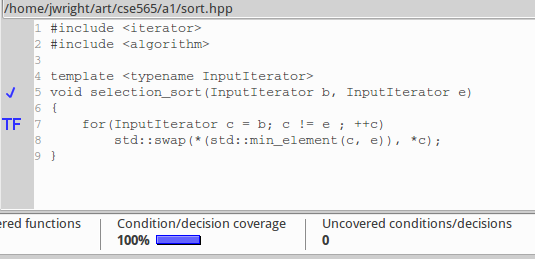
\includegraphics[width=0.8\columnwidth]{100percent_coverage.png}
    \caption{Decision Coverage Results shows 100\% from the existing randomized
        tests,}
    \label{fig:sort_coverage}
\end{figure}

\subsection{Testing a bigger project}
To better evaluate the strength of these tools, and in an effort to elicit an
A from Professor Dasgupta, I applied Decision Coverage to this semester's CSE
531 project.  Listing~\ref{lst:q_h} shows the implementation submitted for
grading.  Listing~\ref{lst:q_test_cpp} shows the unit test code prior to
analyzing coverage. 

\begin{figure}
    \centering
    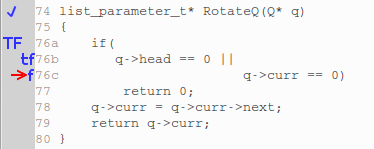
\includegraphics[width=0.8\columnwidth]{missed_decision_coverage.png}
    \caption{Decision Coverage Results show that {\tt RotateQ()} is never called
    with {\tt q->curr == 0} being true}
    \label{fig:decision_coverage_before}
\end{figure}

Figure~\ref{fig:decision_coverage_before} shows the coverage with some
opportunity for improvement. Notice that this current test suite achieves 100%
statement coverage, thus a simpler tool such as Visual Studio's coverage
analysis or gcc's gcov would say this software is 100\% covered. With these
tools one can make that dangerous decision that he is done testing.
BullseyeCoverage is a decision/condition tool and
Table~\ref{tab:before_coverage} summarizes the results. 

{\tt InitQ}, {\tt PeekQ} and {\tt size\_} all show N/A for decision coverage
because those functions do not have any decisions.
Figure~\ref{fig:decision_coverage_before} shows that we are missing a test that
evaluates the false condition of line 76c. This condition corresponds to calling
rotate on an empty queue, but with a corrupt head pointer. We can construct
a test for this behavior as shown in Listing~\ref{lst:create_bad_condition}.

\lstinputlisting[language=C++,label={lst:create_bad_condition},caption={New test
to improve condition coverage}]{create_bad_condition.cpp}

Which improves our coverage to 100\% as shown in Figure~\ref{fig:improved_coverage}.

\begin{table}
    \centering
    \caption{Coverage achieve prior to coverage analysis}
    \label{tab:before_coverage}
    \begin{tabular}{ l | c | c}
        \hline
        Function & Fn Coverage & Condition/Decision  \\
        \hline \hline 
        \tt{RotateQ(Q*)}	& 100\%	 & 83\%	 \\
        \tt{AddQ(Q*,list\_parameter\_t*)} &	100\% & 100\%	\\
        \tt{DelQ(Q*)}	& 100\% & 100\% \\	
        \tt{InitQ(Q*)}	& 100\% & N/A \\	
        \tt{PeekQ(Q*)}	& 100\% & N/A \\	
        \tt{size\_(Q*)}	& 100\% & N/A \\	
        \hline
    \end{tabular}
\end{table}

\begin{figure}
    \centering
    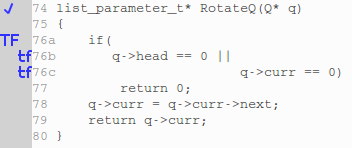
\includegraphics[width=0.8\columnwidth]{improved_decision_coverage.png}
    \caption{Decision Coverage Results show that {\tt RotateQ()} is never called
    with {\tt q->curr == 0} being true}
    \label{fig:improved_coverage}
\end{figure}

To corroborate these results I found another tool called Squish, from a company
froglogic \autocite{_froglogic_????}. The website has a great deal more polish
and feels to me a more modern tool. The tool is configured in a similar way by
setting an environment variable: {\tt export COVERAGESCANNER\_ARGS=--cs-on}. The
tool ran fine, and generated similar coverage metrics, but this tool was much
less usable. The final coverage result shown in Figure~\ref{fig:squish_coverage}
felt like a more modern UI than bullseye, but the workflow was less usable. 

Bullseye made a very simple extension to the source code by breaking each
condition onto sub lines and numbering the sub-lines with letters, a,b,c etc. The
margin then included the t/f and T/F for each decision and condition
respectively. This is a massively smoother workflow and I can see at a glance
where my tests need to improve. In Squish, one has to mouse over each condition
to see a report of the condition table. This table is readable, but its slow to
mouse over each condition. I preferred the Bullseye tool.

\begin{figure}
    \centering
    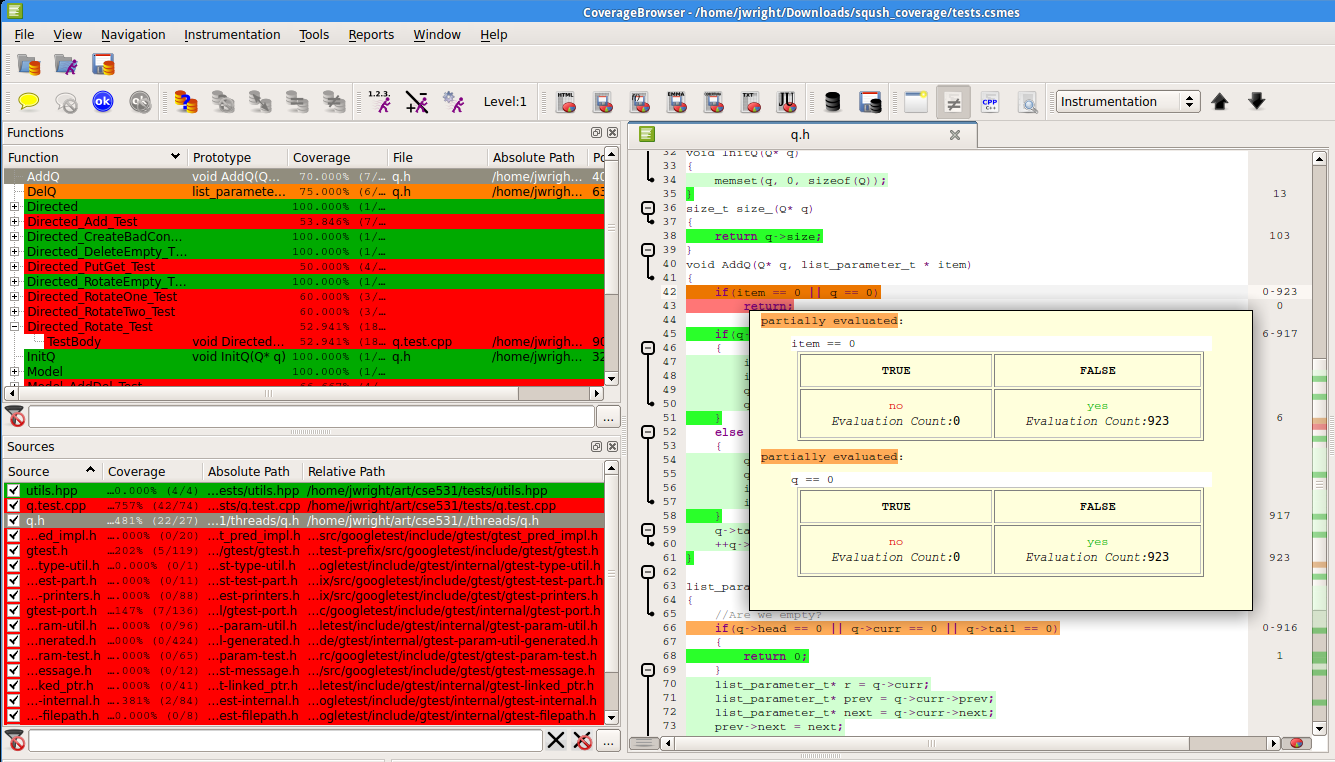
\includegraphics[width=0.8\columnwidth]{Squish.png}
    \caption{Squish coverage tool for C++}
    \label{fig:squish_coverage}
\end{figure}

\section{Static Analysis}

For static analysis, I looked at two tools. CppCheck \autocite{_cppcheck_????}
a free analysis tool, and Coverity \autocite{_software_coverity}. Coverity is
available for free to open source projects via github.  Each tool required some
configuration before final analysis. Table~\ref{tab:analysis_types} summarizes
the types of analysis done by each tool.

\begin{table}
    \centering
    \caption{Type of analysis}
    \label{tab:analysis_types}
    \begin{tabular}{ l | c | c }
        \hline
        Level              & Coverity   & CppCheck \\
        \hline \hline
        Free             & Open Source Only & \checkmark  \\
        Style            & \checkmark & \checkmark \\
        Missing Include  & \checkmark & \checkmark \\
        Performance      & \checkmark & \checkmark  \\
        Portability      & \checkmark & \checkmark  \\
        Unused Functions & \checkmark & \checkmark  \\
        General Warnings & \checkmark & \checkmark  \\
        Flow Analysis    & \checkmark &   \\
        \hline
    \end{tabular}
\end{table}



\subsection{Coverity}
Using github, Coverity is accessible via the travis build engine. Thus one
simple needs to setup travis and Coverity scan is available.
Listing~\ref{lst:travis_build} shows a sample configuration script that will
build a C++ application, and push the results to Coverity.
\lstinputlisting[label={lst:travis_build},caption={Configuration
file for Coverity on Github}]{travis.yml} 
Figure~\ref{fig:travis-ci} shows an example build using the Travis continuous
integration system. 
\begin{figure}
    \centering
    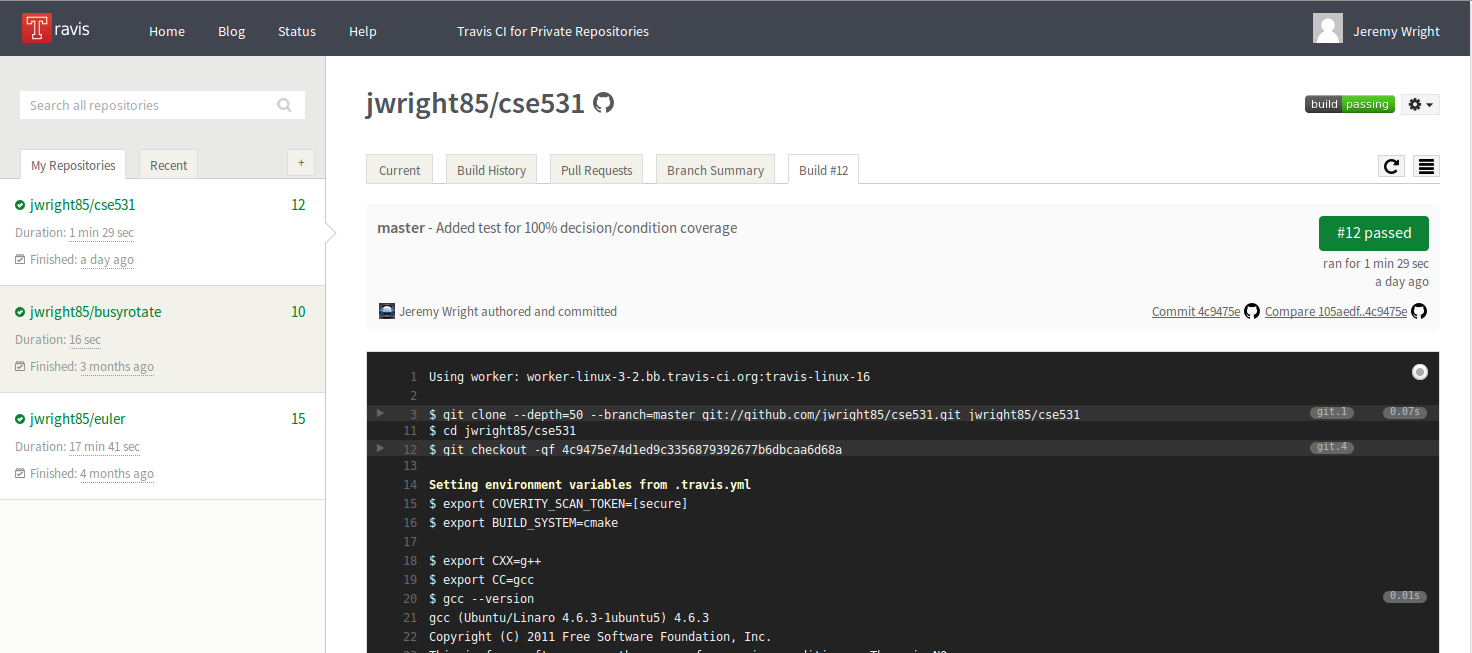
\includegraphics[width=0.8\columnwidth]{AutomatedBuild.png}
    \caption{Automated from Travis-ci automatically pushes build to Coverity for
    analysis.}
    \label{fig:travis-ci}
\end{figure}

Once the build is complete, Travis pushes the build results to Coverity for
analysis. Figure~\ref{fig:coverity_results} shows the results of such a scan.
Coverity was unable to find any errors in the static analysis.

\begin{figure}
    \centering
    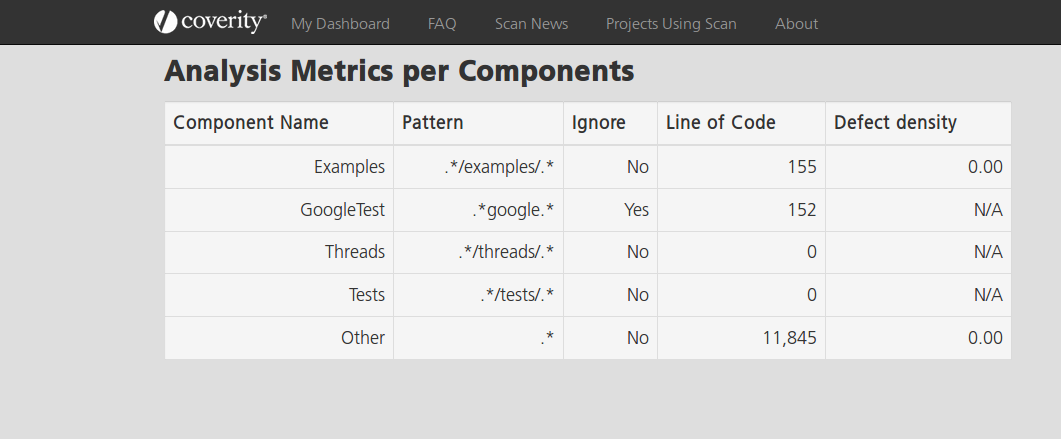
\includegraphics[width=0.8\columnwidth]{CoverityScan.png}
    \caption{Scan Results from Coverity}
    \label{fig:coverity_results}
\end{figure}

\subsection{CppCheck}
Similarity cppcheck is an command line tool that can statically analyze source
code. The tool is configured simply as in Listing~\ref{lst:cppcheck_result}.
Running this on the CSE 531 project agreed with Coverity that no issues
existed. 
\lstinputlisting[language=bash,label={lst:cppcheck_result},caption={CppCheck
Output for CSE 531 project.}]{cppcheck_result.log}

Instead of giving up, I ran cppcheck on the test code to see if it found any
issues. The test code in fact did have an uninitialized bug as shown by
Listing~\ref{lst:cppcheck_test_code}.
\lstinputlisting[language=bash,label={lst:cppcheck_test_code},caption={CppCheck
Output for CSE 531 project.}]{cppcheck_test.log} Listing~\ref{lst:test_code}
shows the minimized uninitialized bug. 
\lstinputlisting[language=C,label={lst:test_code},caption={Test code for
CSE531}]{cppcheck_test_code.c}

I then fixed the test code in Listing~\ref{lst:fixed_test_code}. Final analysis
in Listing~\ref{lst:fixed_test_code_result} shows no outstanding problems.

\lstinputlisting[language=C,label={lst:fixed_test_code},caption={Fixed Test code}]{cppcheck_test_code_fixed.c}
\lstinputlisting[language=bash,label={lst:fixed_test_code_result},caption={Final analysis}]{cpp_fixed_result}

\subsubsection{Injecting Error}
To further evaluate cppcheck we can inject errors into the application and
verify cppcheck can find them.  Starting with the selection sort code in
Listing~\ref{lst:sort}, we can inject three issues, an uninitialized variable,
an unused variable, and a mixed pointer/value type declaration. This results in 
Listing~\ref{lst:sort_broken}.  

\lstinputlisting[language=C++,label={lst:sort_broken},caption={Injected faults
for Selection Sort Implementation}]{sort_broken.hpp}

This results in 2 faults shown in Listing~\ref{lst:broken_cppcheck}
\lstinputlisting[language=bash,label={lst:broken_cppcheck},caption={Analysis of
broken code}]{broken.cppcheck}
I am however disappointed with the results. The these faults didn't show
anything that the compiler won't show with high a high warning level set.
Additionally it missed the severe style issue of declaring a pointer and in
integer on the same line.  

\section{Conclusion}
Decision/Condition coverage is a fantastic tool for identifying areas where unit
tests are falling short. In my own code the randomized testing experiments are
greatly augmented by this analysis. I attempted to acquire a license to
Testwell's CTC++ test tool which provide Multiple condition coverage. The
company, however,  wouldn't provide an evaluation
license. 

Static analysis is also a strong tool that augments the compiler's own warning
reports. I have a habit of compiling with warnings as errors, and this resulting
in static analysis finding very little. On a larger code base, static analysis
will certainly show greater value. Coverity has a leg up on Cppcheck for the
depth of it's analysis. However for this simplified test case CppCheck found
more issues. Its certainly a case where both tools augment each other.

\clearpage
\printbibliography

\clearpage
\section{Listings}
\lstinputlisting[language=C++,label={lst:q_h},caption={Queue Implementation for
CSE531}]{q.h}
\lstinputlisting[language=C++,label={lst:q_test_cpp},caption={Initial Test code for CSE531}]{q.test.before.cpp}



\end{document}

